\subsection{Numeric convergence based on dimensionality}
\label{app:numconv}

\begin{figure}
\centering
\subfigure{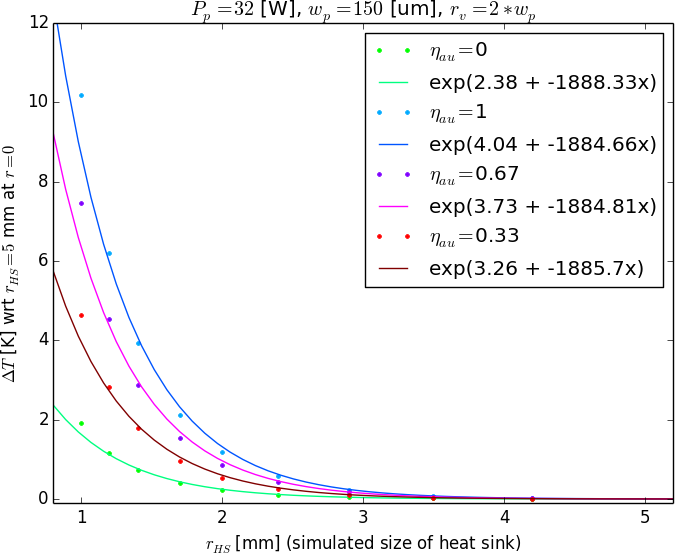
\includegraphics[width=7cm]{img/appendix/r_HS-vs-T.png}}
\subfigure{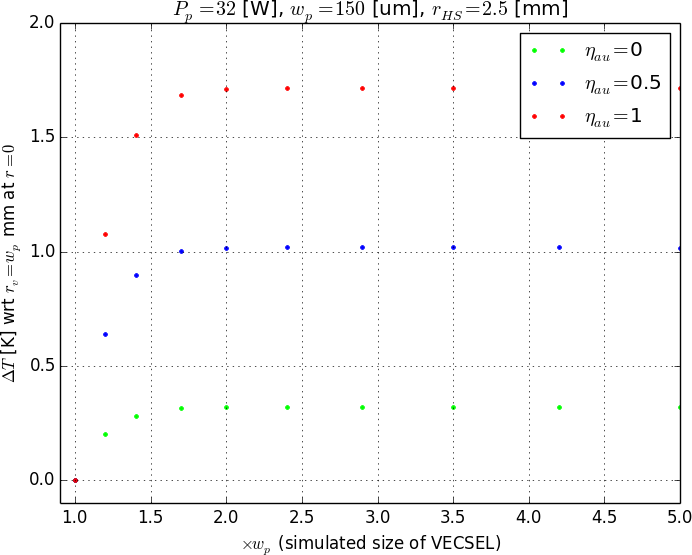
\includegraphics[width=7cm]{img/appendix/r_v-vs-T.png}}
\caption{Left: Investigating on the convergence of the result,
depending on the system's dimension.
The size considered for the heat sink
is exponentially important.
Right: Investigating on the convergence of the result,
depending on the dimension of the VECSEL.
Considering a system larger than $2w_\mathrm{p}$
doesn't influence the over all result.}
\label{img:r_HS-r_v-vs-dT}
\end{figure}

Measuring the performance of a sample
in an experiment
is not the same as simulating it
numerically.
With COMSOL we can exploit
certain symmetries
imposed by the structure.
One is the radial symmetry
around an irradiated spot,
so that COMSOL has to solve
the equations only in two
rather than three dimensions --
which speeds up the calculations.
A second common simplification
is to simulate the VECSEL dimensions
only up to twice the size
of the pump spot \cite{Kemp2008}.
In order to ensure
such simplifications
don't lead to wrong conclusions,
we have to investigate
on the convergence behavior
depending on these parameters.
The names of parameters
are taken from
appendix~\ref{app:comsol_deriv:Q}--\ref{app:comsol_deriv:impl}
and Tab.~\ref{tab:comsolparams}.

Figure~\ref{img:r_HS-r_v-vs-dT} (left) presents
the convergence of the numerical result
depending on the system's size.
Each data point represents the following:
I simulate the temperature
on the surface of the structure
caused by a $P=32\,\mathrm{W}$,
$2w_p=300\,\mu\mathrm{m}$ pump diameter beam.
The radius of the VECSEL
is held constant at
$r_\mathrm{v}=2w_\mathrm{p}$.
In the center (at $r=0$)
the temperature is the highest;
this is the value we store,
for each system size $r_\mathrm{HS}$;
the considered radius of the heat sink.
For different values of $\eta_\mathrm{au}$
I look at various radii between
$r_\mathrm{HS}=1\,\mathrm{mm}$
and $r_\mathrm{HS}=5\,\mathrm{mm}$
(twice the size of our actual structure
with a cross section of $5\times5\,\mathrm{mm}^2$).
In the plot $\Delta T$ refers to the difference
between the temperature obtained with
the $r_\mathrm{HS}$ specified along the x-axis
and the temperature with $r_\mathrm{HS}=5\,\mathrm{mm}$.

The larger $r_\mathrm{HS}$ is chosen,
the less relevant is its actual value --
the temperature spread due to the extra bulk material
goes exponentially.
Therefore,
it seems to be important
to simulate the heat sink
(diamond layer and copper bulk)
as its full size.
The size of the VECSEL on the other hand
seems to be far less important;
its over all volume
and thus its ability to store and transfer heat
is small.
VESCEL sizes larger than two times the beam radius
result in the same temperature increase.
This statement is visualized
in Fig.~\ref{img:r_HS-r_v-vs-dT} (right).
In this plot,
the heat sink is kept
at constant $r_\mathrm{HS}=2.5\,\mathrm{mm}$ and
$r_\mathrm{v}$ is varied as multiples of $w_\mathrm{p}$.

The influence of the considered thickness of the gold layer
depends on whether or not
the incident beam is absorbed in this interface --
i.e. whether the gold layer only conducts the heat,
or is itself a heat source.
Figure~\ref{img:t_au-t_HS-vs-dT} (left)
illustrates this consideration.

\begin{figure}
\centering
\subfigure{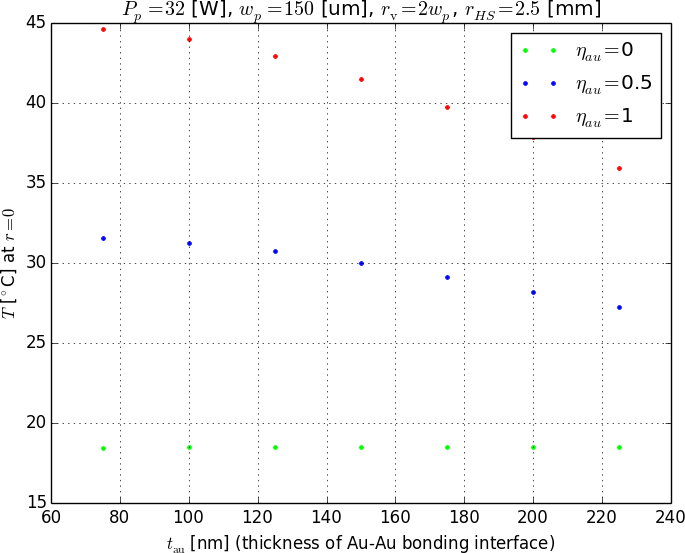
\includegraphics[width=7cm]{img/appendix/t_au-vs-T.png}}
\subfigure{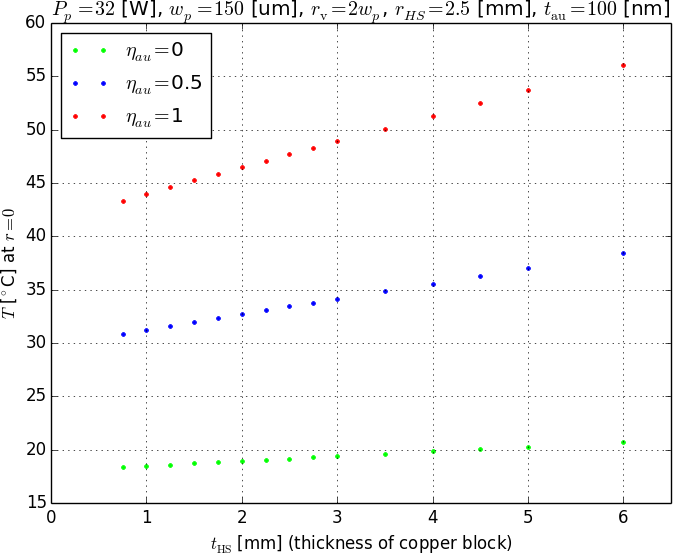
\includegraphics[width=7cm]{img/appendix/t_HS-vs-T.png}}
\caption{Left: Investigating on the convergence of the result,
depending on the thickness of the Au-Au bonding interface.
If we assume the gold layer
absorbs at least some of the incident beam,
we have to know the thickness of this layer.
Right: Investigating on the convergence of the result,
depending on the thickness of the copper heat sink considered.
Its importance depends on whether or not
we assume the gold layer to act as a heat source.}
\label{img:t_au-t_HS-vs-dT}
\end{figure}

In order to look at the influence of
the heat sink copper block
we assume
$r_\mathrm{HS}=2.5\,\mathrm{mm}$,
$r_\mathrm{v}=2w_\mathrm{p}$,
$t_\mathrm{au}=100\,\mathrm{nm}$.
The bottom boundary of the copper block
is held at constant temperature.
A thicker copper heat sink hence means
that the heat has to travel a longer distance.
As shown in Fig.~\ref{img:t_au-t_HS-vs-dT} (right)
this extra distance is relevant;
especially if we consider the gold layer
to act as a heat source.

